
\section{Preliminaries}
\label{sec:prelim}

% Current structure: (1) define G and T, per-packet delay, (2) example scenario, (3) unicast flow definition, (4) multicast flow definition, (5) multicast implementation, (6) multiple link failures

In this section, we provide the necessary background to describe our algorithms in Section \ref{sec:algs}. First, we describe some PMU applications and their QoS requirements 
(Section \ref{subsec:pmu-requirements}).  Then, we present a motivating example referenced throughout this document (Section \ref{subsec:problem-scenario}).
Section \ref{subsec:notation} defines terms and notation.  We give an overview of OpenFlow in Section \ref{subsec:openflow} and Section \ref{subsec:basic} details
our OpenFlow multicast implementation.


\subsection{PMU Applications and Their QoS Requirements} 
\label{subsec:pmu-requirements}

In this work, we consider the design of a communication network for disseminating critical Smart Grid data, principally data associated with PMU applications.  Here
we detail the QoS requirements of a few of these applications, with a particular emphasis on PMU applications with the most stringent E2E delay requirements.
%such as wide-area control and system protection (SIPS). 
Table \ref{tab:app-requirements} shows packet delay and frequency requirements of three PMU applications, each described below.
%We briefly describe each application below.


%starting with Table \ref{tab:app-requirements} that details packet delay and frequency requirements of three PMU applications.
%The QoS requirements of several PMU applications are presented in Table \ref{tab:app-requirements}.  
%Some of these applications (i.e., SIPS and distributed wide area control) have already been deployed on power grids worldwide. 
%In this work, we focus on PMU applications with the most stringent E2E delay requirements, such as closed-loop control and system protection (SIPS).
%We briefly describe each application below.
System Integrity Protection Scheme (SIPS) applications ensure that the entire power grid remains in a healthy state after local power grid machines (e.g., relays) 
have taken mitigating actions to remedy local emergencies.  
To do so, SIPS applications require accurate and timely PMU measurements to identify system instability and to take correct mitigating actions (e.g., trip power generation) \cite{Bakken11}.
%at small time scales (within $50-250$ ms).



Islanding is a safety measure commonly used in power systems that separates entire sections (i.e., the island) of the power grid from the larger system in periods of voltage and frequency 
instability.  Due to a lack of real-time situational awareness, power grid operators and oversight bodies mandate a conservative approach of disconnecting all distributed generation sources 
(e.g., wind and solar) from a locally islanded system. PMU measurements can provide the situational awareness to enable less wasteful islanding practices. Moreover,
as distributed generation increases (as is the current trend), simultaneously disconnecting large number of generation sources will actually further destabilize the grid.  
PMUs are critical to future anti-islanding applications that will
use PMU data to determine when distributed generation sources can safely remain online and thereby help preserve power grid stability \cite{Bakken11}.
%future, the solution will be to keep these DG sources online.  To do so, PMUs are needed to provide a wide-area view of the grid along with the granular measurements to determine when DG sources can 
%remain online.  This is referred to as anti-islanding \cite{Bakken11}.
%PMUs can provide the wide-area view of the grid along with the granular measurements to determine if distributed generation (DG) sources can remain online.  This will become increasingly important as DG grows because disconnecting a large number of generation sources will actually further de-stablize (rather than stablize the system with current DG penetration levels).necessary 

Wide-area control is a more general category of PMU applications, referring to applications that gather PMU data from disparate sources to determine the health of the power grid 
and initiate control actions, both in real-time.
%PMUs have the capabability to enable wide-area control of the power grid.  
For example, Southern California Edison \cite{Johnson07} measures (using PMUs) and controls voltage at remote locations to ensure voltage safety limits are met for its bulk energy transfers.
Another wide-area control application uses PMUs to measure, detect, and dampen inter-area oscillations in real-time\cite{Bakken11}.

\begin{table}[t]
\begin{center}
\begin{tabular}{|l|l|l||} 
\hline
   	{\bf PMU Application} & {\bf E2E Delay} & {\bf Rate (Hz)} \\ 
		  \hline \hline
		
			SIPS & $8-16$ ms & $120-720+$ \\ 
			Wide Area Control  & $5-50$ ms & $1-240$ \\
			Anti-Islanding  & $5-50$ ms & $30-720+$  \\
			\hline
			\end{tabular}
			\end{center}
\caption{PMU applications and their QoS requirements \cite{Bakken11}.  The end-to-end (E2E) delay requirement is \emph{per-packet}, as advocated by Bakken et al. \cite{Bakken11}.} 
\label{tab:app-requirements}
\end{table}

%\textit{state than nothing is published regarding tolerance to packet loss.}


\subsection{Motivating Example}
\label{subsec:problem-scenario}

Here we present a motivating example to highlight different aspects of the problem addressed in this work.  This example is used throughout the document to help describe our algorithms.
%for fast recovery from link failures. 
%all three aspects of our solution: 
%In this work, we address the problem of detecting failed communication links used to dissemtinate critial PMU data, computing backup trees that avoid failed links, 
%and the quick installation of these backup trees.  %Collectively, the aim is to minimize the disruption caused by faulty links. % through fast detection and 
%To build better intuition for the problem we provide an example scenario.

%Figure \ref{fig:intuition-example} shows two PMUs, one at $b$ and other at $c$, that produce PMU measurements at a fixed rate and are disseminated by two separate source-based multicast trees $T_b$ and $T_c$.  
Figure \ref{fig:intuition-example} shows two source-based multicast trees used to disseminate PMU measurement data produced by a PMU at $b$ and another at $c$. $T_b$, shown in green, 
is rooted at $b$ and disseminates $b$'s PMU data to its leaf nodes (i.e., data sinks) $\{p,q,r,s\}$. The blue tree, $T_c$, multicasts $c$'s PMU measurements to its
leaf nodes $\{r,s,t,u,v\}$.  %$T_b$ nodes are green, $T_c$ nodes are blue, and half-green/half-blue nodes are in both $T_b$ and $T_c$.  
Half-green/half-blue nodes are in both $T_b$ and $T_c$.   Before any link failures occur, the original multicast trees (Figure \ref{fig:intuition-example-t1}) meets the delay requirements
specified by each data sink.  
%We assume that each data sink specifies an end-to-end per-packet delay requirement.
%The original multicast trees, shown in Figure \ref{fig:intuition-example-t1}, meets all delay requirements.  %until link $(g,l)$ fails (e.g., loss rate exceeds a threshold). 

At some point, link $(g,l)$ fails (e.g., its loss rate exceeds a threshold or it goes completely offline).
This prevents $p,q,r$ and $s$ from receiving any packets from either $T_b$ or $T_c$ until each multicast tree is repaired, leaving the delay requirement of each these sink nodes unsatisfied. 
Figure \ref{fig:intuition-example-t2} shows two backup multicast trees -- one for $T_b$ and the other for $T_c$ --
installed after it is detected that $(g,l)$ has failed.
Notice that each backup tree contains no path using the failed link, $(g,l)$, and has a path between its root and each of its data sinks.
In the coming sections we present algorithms that detect these types of link failures, compute backup multicast trees like the ones shown in Figure \ref{fig:intuition-example-t2}, 
and quickly install these backup trees in order to minimize packet loss and delay.
%to recover from link failures by installing backup multicast trees, similar to the one in Figure \ref{fig:intuition-example-t1}.


%Figure \ref{fig:intuition-example} depicts a scenario where a single link, $(g,l)$, in a multicast tree fails.  %Figure \ref and the resulting repaired tree.
%each data sink specifies a per-packet delay requirement. The multicast tree in Figure \ref{fig:intuition-example-t1} uses link $(b,c)$, which  we assume fails between the
%time the snapshots in Figure \ref{fig:intuition-example-t1} and Figure \ref{fig:intuition-example-t2} are taken.

\begin{figure*}[t]
  \begin{center}
    \subfigure[Original multicast trees $T_b$ (green) and $T_c$ (blue). ]{\label{fig:intuition-example-t1}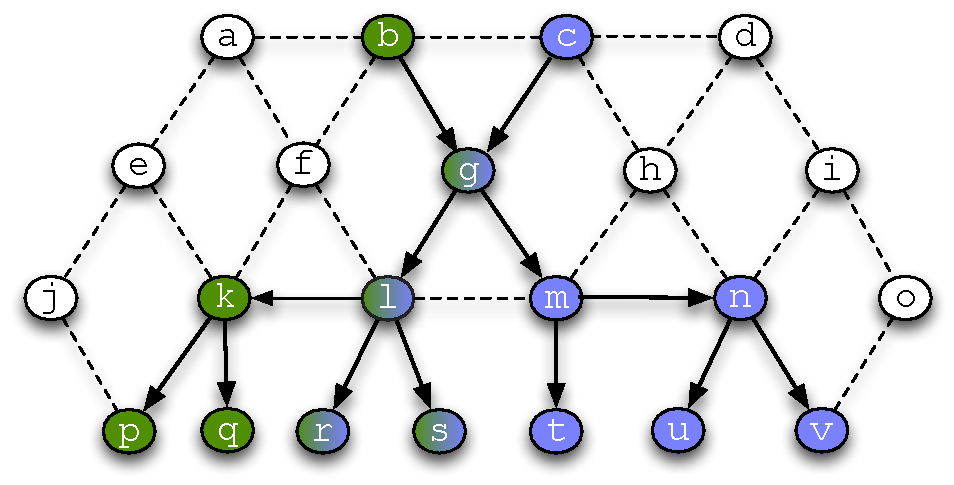
\includegraphics[scale=0.46]{figs/multi-tree-example1.pdf}} 
    \subfigure[Backup multicast trees -- $\hat{T}_b$ and $\hat{T}_c$ for $T_b$ and $T_c$, respectively --  installed after $(g,l)$ fails. Links unique to each backup tree are circled.]
		{\label{fig:intuition-example-t2}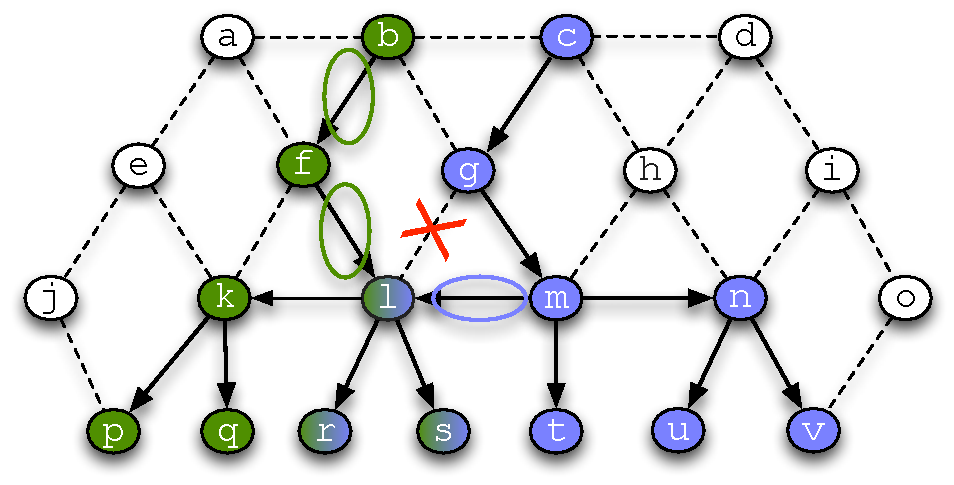
\includegraphics[scale=0.46]{figs/multi-tree-example2.pdf}} 
  \end{center}
\caption{Example problem scenarios with two source-based multicast trees, one rooted at $b$ (in green), $T_b$, and the other at $c$ (in blue), $T_c$. Half-blue/half-green nodes are members of 
both multicast trees. Let $f_b$ and $f_c$ denote the multicast flows corresponding to $T_b$ and $T_c$, respectively.  The multicast trees are shown before and after link $(g,l)$ fails. }
\label{fig:intuition-example}
\end{figure*}


\subsection{Notation and Assumptions}
\label{subsec:notation}


%We model the communication network as a directed graph, $G=(V,E)$, where $V$ consists of three types of nodes: ones that send PMU data (PMU nodes), nodes that receive PMU data (data sinks), 
%and switches connecting PMU nodes and data sinks (typically via other switches). 
We model the communication network as a directed graph $G=(V,E)$, where $(u,d) \in E$ denotes a directed edge from $u$ to $d$ and 
$V$ consists of three types of nodes: ones that send PMU data (PMU nodes), nodes that receive PMU data (data sinks), and switches connecting PMU nodes and data sinks (typically via other switches).
We assume $G$ has $m\geq1$ source-based multicast trees to disseminate PMU data.   Let $T=\{T_1,T_2, \dots ,T_m\}$ refer to the set of $m$ source-based multicast trees in $G$
such that each $T_i = (V_i,E_i,r,S)$ is a tree rooted at $r$ with directed edges $E_i$, vertices $V_i$, and a directed path from $r$ to each $s \in S$.  Let $w(T_i)$ be the total weight of 
all $T_i$ edges.

For convenience, denote $T^l_i = (V^l_i,E^l_i,r,S)$ as the $ith$ directed tree with $l \in E^l_i$.  Associated with each directed tree, $T^l_i$ is a backup tree 
$\hat{T}^l_i=(\hat{V}^l_i,\hat{E}^l_i,r,S)$, a directed tree with root $r$, a directed path from $r$ to each $s \in S$ such that $l \notin \hat{E}^l_i$.  
We refer to  $T^l_i$ and $\hat{T}^l_i$ as a {\em primary tree} and {\em backup tree}, respectively.  In Figure \ref{fig:intuition-example-t2} the two backup trees -- one for $T_b$ and the other for
$T_c$ -- both route around the failed link, $(g,l)$, and have a directed path from its root ($b$ and $c$) to their data sinks ($\{p,q,r,s\}$ and $\{r,s,t,u,v\}$).


%We assume $G$ only contains MTs in $T$. 
%\emph{Packet delay} between a sender, $s$, and receiver, $r$, is the time it takes $s$ to send a packet to $r$.
%Although we are ultimately concerned with meeting the per-packet delay requirements of PMU applications, we use packet loss (as opposed to delay) as an indicator for
%a failed link because OpenFlow provides no native support for timers.
%Note that a data sink's per-packet delay requirement is an end-to-end requirement.

Corresponding to each primary tree, $T_i = (V_i,E_i,r,S)$, is a multicast flow $f_i =(r,S)$ with source, $r$, and data sinks $S=\{d_1, d_2, ... d_k\}$. Each $d_i \in S$ has an end-to-end per-packet
delay requirements and loss rate requirement (specified as the maximum tolerable loss rate of each $e \in E_i$).
Let $F$ be the set of all multicast flows in $G$. 

%\yy{Additionally, a multicast flow, $f_m$, sends packets at the maximum rate of the downstream sink nodes among the unicast flows $f_m$ represents. }

Lastly, we make the following simplifying assumptions:
\begin{itemize}

	\item Before any link fails, we assume that all packets (of PMU data) are correctly delivered such that each data sink's per-packet delay and loss requirements are satisfied.

	\item All sinks have the same same per-packet delay and loss rate requirements.  

	\item We consider the case where multiple links fail over the lifetime of the network but assume that only a \emph{single link fails at-a-time}.

% number of links in tree satisfies delay requirement + loss requirement 

\end{itemize}


\subsection{OpenFlow}
\label{subsec:openflow}

%Our algorithms designs leverage the abstractions provided by software-defined networking as embodied by OpenFlow. 
Our algorithms are built using OpenFlow abstractions and features. Here we provide a brief overview of OpenFlow, with a particular emphasis on the features used by our algorithms.

OpenFlow is an open standard that cleanly separates the control and data planes, and provides a programmable (and possibly centralized) control framework \cite{OpenFlow08}.
All OpenFlow algorithms and protocols are managed by a (logically) centralized controller, while network switches (as their only task) forward packets according to the 
forwarding rules installed by the controller.  
%By building a network-wide view at the controller, control and management algorithms are greatly simplified because they can run as 
%centralized algorithms rather than as slow, error-prone distributed computations executed among network switches and routers.  
%Because our algorithms for computing and installing backup trees in response to link failures are run at the controller, they are simplified in this manner. 

OpenFlow exposes the flow tables of its switches, allowing the controller to add, remove, and delete flow entries, which determine how switches 
forward, copy, or drop packets associated with a controller-managed flow. We use the terms ``flow entry'' and ``forwarding rule'' interchangeably in this document.

OpenFlow switches follow a ``match plus action'' paradigm \cite{OpenFlow08}, in which each switch \emph{matches} an incoming packet based on its header fields
to a flow table table entry and then \emph{actions} (e.g., forward packet, drop packet, copy packet, or modify packet header fields) are applied to the packet as encoded in the flow entry instructions.  
Switches maintains per-flow statistics (e.g., packet counter, number of bytes received, time the flow was installed) that can 
can be queried by the controller.  These statistics are key to our algorithm for detecting packet loss (Section \ref{subsec:pcnt}).

Several of our algorithms use OpenFlow to modify packet headers to customize forwarding and other actions in parts of the network.  We write identifiers in unused packet
header fields to customize the set of actions applied to packets carrying specific identifiers.
We refer to these identifiers as \emph{tags}.  Tags are an abstraction we use to measure packet loss rates (\pcnt in Section \ref{subsec:pcnt}), 
pre-install backup tree flow entries (\pre in Section \ref{subsec:install-backups}), and consolidate flow entries that have common forwarding state (\merge in Section \ref{subsec:merge}).
 %Many of our algorithms write identifiers in unused packet header fields to customize the set of actions %applied to packets carrying an identifier along portions of the network. 
%The ability to modify packet headers is a handy tool used by many of our algorithms to indentify specific packets and customize the actions applied these packets at specific network
%switches.  At network subgraphs, we write an identifier in an unused packet header field, which is used to customerize forwarding or simply indentify packets as they pass through the subgraph.
%We find the ability to modify packet headers especially useful. Many of our algorithms write identifiers in unused packet header fields to induce custom behacior (forwarding) along 
%portions of the network. %network switches induce custom forwarding logic at a subset of multicast tree nodes. 

%ability to manipulate switch forwarding tables and to query switches for per-flow statistics are both fundamental our algorithmfor detecting packet loss inside the network of switches (Section \ref{subsec:detection}).


Measurement studies from the literature \cite{Curtis11,Rotsos12} have identified significant hardware limitations in OpenFlow switches.
%Important hardware limitations  in OpenFlow switch hardware have been reported in the literature \cite{Curtis11,Rotsos12}. 
OpenFlow switches can only support a limited number of flow entries because they 
rely on expensive TCAM memory to perform wildcard matching.  For example, the HP5406zl switch supports approximately $1500$ OpenFlow rules \cite{Curtis11} and the Pronto 3290 switch
can handle $1919$ flow entries \cite{Ferguson13}. 
Another major limitation is control plane bandwidth: OpenFlow switches has been found to be four orders of magnitude less than data plane 
forwarding bandwidth \cite{Curtis11}. This limited bandwidth, along with their slow control/management CPUs, limits the rate in which flow entries can be installed.  
Our simulation study (Section \ref{sec:evaluation}) shows the tangible effects these hardware limitations have on our algorithms (especially \pcnts).
%To date, limitations in OpenFlow switch hardware suffer from some hardware limitations.
%A key OpenFlow limitation is that OpenFlow switches can support a limited number of flow entries because they rely on expensive TCAM memory to perform wildcard matching.  
%For example, the HP5406zl switch supports approximately $1500$ OpenFlow rules \cite{Curtis11} and the NEC PF5820 switch can handle about $750$ flow entries \cite{PF5820}.
%Our simulation study (Section \ref{sec:evaluation}) shows

\subsection{Multicast Implementation} 
\label{subsec:basic}

In keeping with its role as a general framework that provides primitives for programmable networks, OpenFlow does not explicitly provide an implementation for multicast. 
Instead, we design our own multicast implementation called \bases.  \base assign a multicast IP address to each multicast group and use
this address to setup the flow tables at the multicast tree switches.  
  \footnote{Because multicast group membership is static for power grid applications (Section \ref{subsec:pmu-requirements}, 
  we simply determine the members of each multicast group by reading their static assignment from a text file.  Note that if dynamic group membership were to be required, we could 
  replace this static policy using a protocol like IGMP. }

After the controller computes a multicast tree (described in Section \ref{subsec:min-control}), $T_i = (V_i,E_i,r,S)$, \base installs a flow entry at each switch in $V_i$. The flow entry
matches packets using the group's multicast address (all other field are left as wildcards) and sends a copy of each packet out the ports corresponding to the switch's 
outgoing links in $E_i$. If a switch in $E_i$ is adjacent to a downstream host, $h_j$, in the multicast group, then the flow entry rewrites the destination layer 2 and 3 addresses of the 
packet copy sent to $h_j$ to $h_j$'s layer 2 and 3 addresses.
\footnote{Our initial plan was to use the group table abstraction described in the OpenFlow 1.1 specification \cite{OpenFlowSpec1.1} to implement multicast but, unfortunately,
as of the writing of this paper, this feature is not yet supported by the POX controller \cite{Pox} used to implement our algorithms and 
the Mininet emulator \cite{Lantz10} used in our simulations.}

% (1) mcast group assigned mcast address, (2) After mcast tree computed for mcast group, use dst address to match packets at each switch.  packets fwded out the ports corresponding to
%  tree links, rewrite address at leaf switches.  (action applied for leaf's outport)

%those of its adjacent downstream host. (these fields were previously populated with the multicast addresses).




%Another way to implement multicast in OpenFlow is to leverage existing IP multicast protocols as detailed by Kotani et al. \cite{Kotani12}.  
%In this approach, the controller assigns a unique group ID to each multicast tree and creates a group table entry, that uses the group ID, at each switch along the multicast tree.  
%Meanwhile, the sender and its first-hop switch use IGMP to set up and manage the controller-generated group IDs. Finally, the sender embeds the group ID in each multicast packet's destination 
%field, allowing for each switch in the multicast tree to identify and forward multicast packets appropriately. 


